\chapter{Type4Py: Practical Deep Similarity Learning-Based Type Inference for Python}
\label{ch:t4py}

\blfootnote{This chapter is based on the paper, Mir, A. M., Latoškinas, E., Proksch, S., \& Gousios, G., Type4py: Practical Deep Similarity Learning-based Type Inference for Python. In Proceedings of the 44th International Conference on Software Engineering (ICSE'22) (pp. 2241-2252).~\cite{mir2022type4py}.
}

\newcommand{\name}{\tool{Type4Py}}
\newcommand{\cmark}{\ding{51}}
\newcommand{\xmark}{\ding{55}}

\begin{abstract}
Dynamic languages, such as Python and Javascript, trade static typing for 
developer flexibility and productivity. Lack of static typing can cause run-time exceptions and is a
major factor for weak IDE support. To alleviate these issues, PEP 484 introduced
optional type annotations for Python. As retrofitting types to existing
codebases is error-prone and laborious, machine learning (ML)-based approaches have been proposed to
enable automatic type inference based on existing, partially annotated
codebases.
However, previous ML-based approaches are trained and evaluated on human-provided type annotations, 
which might not always be sound, and hence this may limit the practicality for real-world usage.
In this chapter, we present \name, a deep similarity learning-based hierarchical neural network model.
It learns to discriminate between similar and dissimilar types in a high-dimensional space, which results in clusters of types.
Likely types for arguments, variables, and return values can then be inferred through the nearest neighbor search.
Unlike previous work, we trained and evaluated our model on a \emph{type-checked} dataset and used mean reciprocal rank (MRR) to reflect the performance perceived by users.
The obtained results show that \name achieves an MRR of 77.1\%, which is a substantial improvement of 8.1\% and 16.7\% over the state-of-the-art approaches \tool{Typilus} and \tool{TypeWriter}, respectively. Finally, to aid developers with retrofitting types, we released a Visual Studio Code extension, which uses \name to provide ML-based type auto-completion for Python.
\end{abstract}

\newpage

\section{Introduction}
Over the past years, \emph{dynamically-typed} programming languages (DPLs) have become extremely popular among software developers.
The IEEE Spectrum ranks Python as the most popular programming language in 2021~\cite{ieeespec2019}.
It is known that \emph{statically-typed} languages are less error-prone~\cite{ray2014large} and that static types improve important quality aspects of software~\cite{gao2017type}, like the maintainability of software systems in terms of understandability, fixing type errors~\cite{hanenberg2014empirical}, and early bug detection~\cite{gao2017type}.
In contrast to that, dynamic languages such as Python and JavaScript allow rapid prototyping which potentially reduces development time~\cite{hanenberg2014empirical, stuchlik2011static}, but the lack of static types in dynamically-typed languages often leads to type errors, unexpected run-time behavior, and suboptimal IDE support.

To mitigate these shortcomings, the Python community introduced \emph{PEP 484}~\cite{van2014pep}, which adds optional static typing to Python 3.5 and newer.
Static type inference methods~\cite{hassan2018maxsmt, furr2009static} can be employed to support adding these annotations, which is otherwise a manual, cumbersome, and error-prone process~\cite{ore2018assessing}.
However, static inference is imprecise~\cite{pavlinovic2019leveraging}, caused by dynamic language features or by the required over-approximation of program behavior~\cite{madsen2015static}.
Moreover, static analysis is usually performed on full programs, including their dependencies, which is slow and resource-intensive.

To address these limitations of static type inference methods, researchers have recently employed \emph{Machine Learning} (ML) techniques for type prediction in dynamic languages~\cite{hellendoorn2018deep, malik2019nl2type, pradel2019typewriter, allamanis2020typilus}.
The experimental results of these studies show that ML-based type prediction approaches are more precise than static type inference methods or they can also work with static methods in a complementary fashion~\cite{pradel2019typewriter, allamanis2020typilus}. Despite the superiority of ML-based type prediction approaches, their type vocabulary is small and fixed-sized (i.e. 1,000 types). This limits their type prediction ability for user-defined and rare types. To solve this issue, Allamanis et al.~\cite{allamanis2020typilus} recently introduced \tool{Typilus} which does not constraint the type vocabulary size and it outperforms the other models with small-sized type vocabulary.

While the ML-based type inference approaches are effective, we believe that there are two main drawbacks in the recent previous work~\cite{pradel2019typewriter, allamanis2020typilus}:
\begin{itemize}
	\item The neural models are trained and evaluated on developer-provided type annotations, which are not always correct~\cite{ore2018assessing, rak2020python}. This might be a (major) threat to the validity of the obtained results. To address this, a type checker should be employed to detect and remove incorrect type annotations from the dataset.
	\item Although the proposed approaches~\cite{pradel2019typewriter, allamanis2020typilus} obtain satisfying performance for Top-10, it is important for an approach to give a correct prediction in Top-1 as developers tend to use the first suggestion by a tool~\cite{parnin2011automated}. Like the API recommendation research~\cite{liu2018effective, he2021pyart}, the Mean Reciprocal Rank (MRR) metric should also be used for evaluation, which \emph{partially} rewards an approach where the correct API is not in the Top-1 suggestion.
\end{itemize}

Motivated by the above discussion, we present \name, a type inference approach based on \emph{deep similarity learning} (DSL).
The proposed approach consists of an effective hierarchical neural network that maps programs into \emph{type clusters} in a high-dimensional feature space.
Similarity learning has, for example, been used in Computer Vision to discriminate human faces for verification~\cite{chopra2005learning}. Similarly, \name learns how to distinguish between different types through a DSL-based hierarchical neural network.
As a result, our proposed approach can not only handle a very large type vocabulary, but also it can be used in practice by developers for retrofitting type annotations.
In comparison with the state-of-the-art approaches, the experimental results show that \name obtains an MRR of 77.1\%,
which is 8.1\% and 16.7\% higher than \tool{Typilus}~\cite{allamanis2020typilus} and \tool{TypeWriter}~\cite{pradel2019typewriter}, respectively.

\smallskip
\noindent
Overall, this paper presents the following main contributions:
\begin{itemize}
	\item \name, a new DSL-based type inference approach.
	\item A \emph{type-checked} dataset with 5.1K Python projects and 1.2M type annotations. Invalid type annotations are removed from both training and evaluation.
%	\item Different from previous work~\cite{pradel2019typewriter, typilus}, we evaluate the type inference neural models with the MRR metric as well, which considers the rank of predicted type annotations.
	\item A Visual Studio Code extension~\cite{vscodet4py}, which provides ML-based type auto-completion for Python.
\end{itemize}

To foster future research, we publicly released the implementation of the \name model and its dataset on Zenodo.\footnote{https://doi.org/10.5281/zenodo.5913787}

The rest of the chapter is organized as follows. Section \ref{ch4:sec:rw} reviews related work on static and ML-based type inference. The proposed approach, \name, is described in Section \ref{ch4:sec:pa}. Section \ref{ch4:sec:data} gives details about the creation of the type-checked dataset for evaluation. The evaluation setup and empirical results are given in Section \ref{ch4:sec:es} and Section \ref{ch4:sec:eval}, respectively. Section \ref{ch4:sec:prac} describes the deployment of \name and its usage in Visual Studio Code. Section \ref{ch4:sec:discuss} discusses the obtained results and gives future directions. Finally, we summarize our work in Section \ref{ch4:sec:sum}.

\newpage

\section{Related Work}\label{ch4:sec:rw}

\begin{table*}[!t]
	\centering
	\caption{Comparison between \name and other learning-based type inference approaches}
	\label{tab:comp-learning-appr}
	\begin{threeparttable}
	\resizebox{\textwidth}{!}{\begin{tabular}{c c c c c c c c c c}
		\toprule
		\multirow{2}{*}{Approach} & \multirow{2}{*}{Size of type vocabulary} & \multirow{2}{*}{ML model} & \multicolumn{3}{c}{Type hints} & &  \multicolumn{3}{c}{Supported Predictions} \\
		\cmidrule{4-6} \cmidrule{8-10}
		& & & Contextual & Natural & Logical & & Argument & Return & Variable \\
		\midrule
		\textbf{\name} & Unlimited & HNN (2x RNNs) & \cmark & \cmark & \xmark & & \cmark & \cmark & \cmark \\
		JSNice \cite{raychev2015predicting} & 10+ & CRFs & \cmark & \cmark & \xmark &&  \cmark & \xmark & \xmark \\
		Xu et al. \cite{xu2016python} & - & PGM & \xmark & \cmark & \cmark & & \xmark & \xmark & \cmark \\
		DeepTyper \cite{hellendoorn2018deep} & 10K+ & biRNN & \cmark & \cmark & \xmark & & \cmark & \cmark & \cmark \\
		NL2Type \cite{malik2019nl2type} & 1K & LSTM & \xmark & \cmark & \xmark &  & \cmark & \cmark & \xmark \\
		TypeWriter \cite{pradel2019typewriter} & 1K & HNN (3x RNNs) & \cmark & \cmark & \xmark & & \cmark & \cmark & \xmark  \\
		LAMBDANET \cite{wei2019lambdanet} & 100\tnote{a} & GNN & \cmark & \cmark & \cmark & & \xmark & \xmark & \cmark \\
		OptTyper \cite{pandi2020opttyper} & 100 & LSTM & \xmark & \cmark & \cmark &  & \cmark & \cmark & \xmark \\
		Typilus \cite{allamanis2020typilus} & Unlimited & GNN & \cmark & \cmark & \xmark  & & \cmark & \cmark & \cmark \\
		TypeBert \cite{jesse2021learning} & 40K & BERT & \cmark & \cmark & \xmark & & \cmark & \cmark & \cmark \\
		\bottomrule
	\end{tabular}}
    \begin{tablenotes}
    	\item[a] {\footnotesize Note that LAMBDANET's pointer network model enables to predict user-defined types \\ outside its fixed-size type vocabulary.}
    \end{tablenotes}
    \end{threeparttable}
\end{table*}

\paragraph{Type checking  and inference for Python}
In 2014, the Python community introduced a type hints proposal \cite{van2014pep} that describes adding optional type annotations to Python programs. A year later, Python 3.5 was released with optional type annotations and the \textit{mypy} type checker \cite{lehtosalo2017mypy}. This has enabled gradual typing of existing Python programs and validating added type annotations. Since the introduction of type hints proposal, other type checkers have been developed such as \textit{PyType} \cite{pytype}, \textit{PyRight} \cite{pyright}, and \textit{Pyre} \cite{pyre}.

A number of research works proposed type inference algorithms for Python \cite{salib2004faster, maia2012static, hassan2018maxsmt}. These are static-based approaches that have a pre-defined set of rules and constraints. As previously mentioned, static type inference methods are often imprecise \cite{pavlinovic2019leveraging}, due to the dynamic nature of Python and the over-approximation of programs' behavior by static analysis \cite{madsen2015static}.

\paragraph{Learning-based type inference} In 2015, Rachev et al.~\cite{raychev2015predicting} proposed JSNice, a probabilistic model that predicts identifier names and type annotations for JavaScript using conditional random fields (CRFs). The central idea of JSNice is to capture relationships between program elements in a dependency network.
However, the main issue with JSNice is that its dependency network cannot consider a wide context within a program or a function.

Xu et al.~\cite{xu2016python} adopt a probabilistic graphical model (PGM) to predict variable types for Python. Their approach extracts several uncertain type hints such as attribute access, variable names, and data flow between variables. Although the probabilistic model of Xu et al.~\cite{xu2016python} outperforms static type inference systems, their proposed system is slow and lacks scalability.

Considering the mentioned issue of JSNice, Hellendoorn et al.~\cite{hellendoorn2018deep} proposed DeepTyper, a sequence-to-sequence neural network model that was trained on an aligned corpus of TypeScript code. The DeepTyper model can predict type annotations across a source code file by considering a much wider context. Yet DeepTyper suffers from inconsistent predictions for the token-level occurrences of the same variable. Malik et al.~\cite{malik2019nl2type} proposed NL2Type, a neural network model that predicts type annotations for JavaScript functions. The basic idea of NL2Type is to leverage the natural language information in the source code such as identifier names and comments. The NL2Type model is shown to outperform both the JSNice and DeepTyper at the task of type annotations prediction~\cite{malik2019nl2type}.

Motivated by the NL2Type model, Pradel et al.~\cite{pradel2019typewriter} proposed the TypeWriter model which infers type annotations for Python. TypeWriter is a deep neural network model that considers both code context and natural language information in the source code. Moreover, TypeWriter validates its neural model's type predictions by employing a combinatorial search strategy and an external type checker. Wei et al.~\cite{wei2019lambdanet} introduced LAMBDANET, a graph neural network-based type inference for TypeScript. Its main idea is to create a type dependency graph that links to-be-typed variables with logical constraints and contextual hints such as variables assignments and names. For type prediction, LAMBDANET employs a pointer-network-like model which enables the prediction of unseen user-defined types. The experimental results of Wei et al.~\cite{wei2019lambdanet} show the superiority of LAMBDANET over DeepTyper.

Given that the natural constraints such as identifiers and comments are an uncertain source of information, Pandi et al.~\cite{pandi2020opttyper} proposed OptTyper which predicts types for the TypeScript language. The central idea of their approach is to extract deterministic information or logical constraints from a type system and combine them with the natural constraints in a single optimization problem. This allows OptTyper to make a type-correct prediction without violating the typing rules of the language. OptTyper has been shown to outperform both LAMBDANET and DeepTyper~\cite{pandi2020opttyper}.

Except for LAMBDANET, all the discussed learning-based type inference methods employ a (small) fixed-size type vocabulary, e.g., 1,000 types. This hinders their ability to infer user-defined and rare types. To address this, Allamanis et al.~\cite{allamanis2020typilus} proposed Typilus, which is a graph neural network (GNN)-based model that integrates information from several sources such as identifiers, syntactic patterns, and data flow to infer type annotations for Python. Typilus is based on metric-based learning and learns to discriminate similar to-be-typed symbols from different ones. However, Typilus requires a sophisticated source code analysis to create its graph representations, i.e. data flow analysis. Very recently, inspired by "Big Data", Jesse et al. ~\cite{jesse2021learning} presented TypeBert, a pre-trained BERT model with simple token-sequence representation. Their empirical results show that TypeBert generally outperforms LAMBDANET. The differences between \name and other learning-based approaches are summarized in Table \ref{tab:comp-learning-appr}.

\newpage
\section{Proposed Approach}\label{ch4:sec:pa}

\begin{figure}[!t]
	\centering
	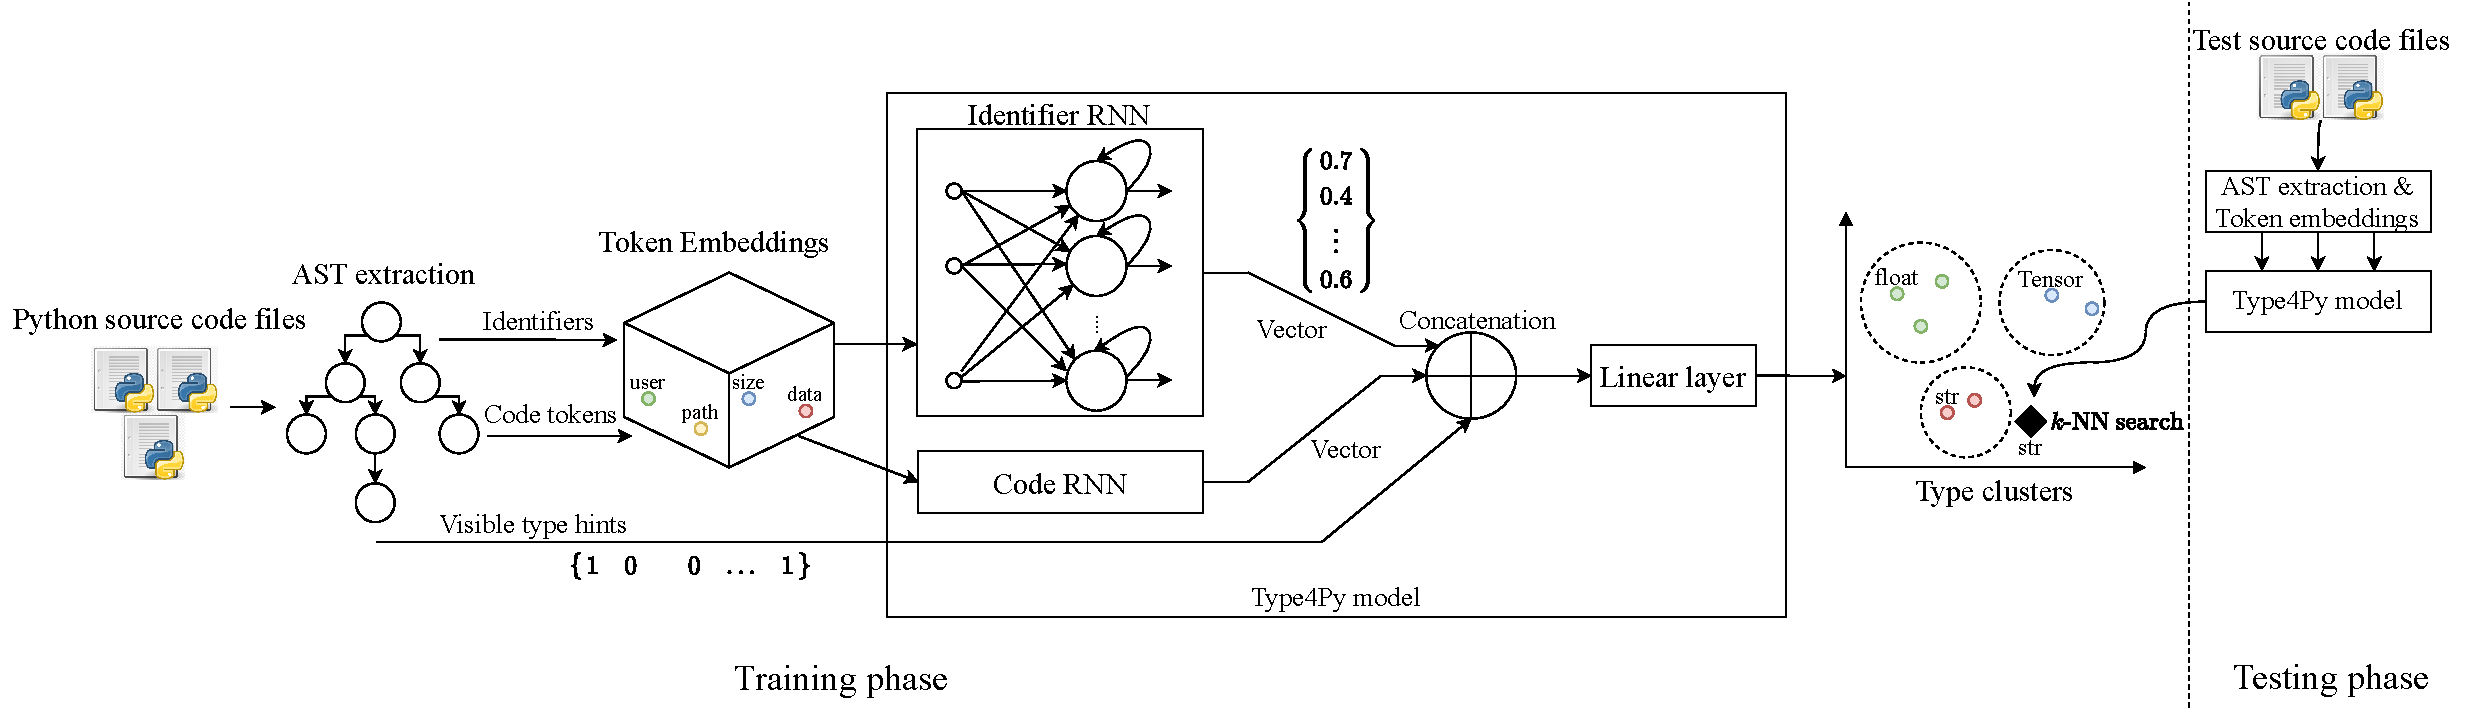
\includegraphics[width=\linewidth]{chapters/ch4/figs/Type4Py-Overview.pdf}
	\caption{Overview of \name approach}
	\label{ch4:fig:overview-approach}
\end{figure}

This section presents the details of \name by going through the different steps of the pipeline that is illustrated in the overview of the proposed approach in Figure~\ref{ch4:fig:overview-approach}.
We first describe how we extract type hints from Python source code and then how we use this information to train the neural model.

\subsection{Type Hints}
We extract the Abstract Syntax Tree (AST) from Python source code files. By traversing the nodes of ASTs, we obtain type hints that are valuable for predicting types of function arguments, variables, and return types. The obtained type hints are based on natural information, code context, and import statements which are described in this section.

\paragraph{Natural Information}
As indicated by the previous work~\cite{hindle2012naturalness, malik2019nl2type}, source code contains useful and informal natural language information that is considered as a source of type hints. In DPLs, developers tend to name variables and functions' arguments after their expected type~\cite{milojkovic2017exploiting}. Based on this intuition, we consider identifier names as the main source of natural information and type hint. Specifically, we extract the name of functions ($N_{f}$) and their arguments ($N_{args}$) as they may provide a hint about the return type of functions and the type of functions' arguments, respectively. We also denote a function's argument as $N_{arg}$ hereafter. For variables, we extract their names as denoted by $N_{v}$.

\paragraph{Code Context}
We extract all uses of an argument in the function body as a type hint.
This means that the complete statement, in which the argument is used, is included as a sequence of tokens. Similarly, we extract all uses of a variable in its current and inner scopes.
Also, all the return statements inside a function are extracted as they may contain a hint about the return type of the function.

\paragraph{Visible type hints (VTH)}
In contrast to previous work that only analyzed the direct imports~\cite{pradel2019typewriter}, we recursively extract all the import statements in a given module and its transitive dependencies.
We build a dependency graph for all imports of user-defined classes, type aliases, and \texttt{NewType} declarations
For example, if module \texttt{A} imports \texttt{B.Type} and \texttt{C.D.E}, the edges (\texttt{A}, \texttt{B.Type}) and (\texttt{A}, \texttt{C.D.E}) will be added to the graph.
We expand wildcard imports like \texttt{from foo import *} and resolve the concrete type references.
We consider the identified types as \emph{visible} and store them with their fully-qualified name to reduce ambiguity. For instance, \texttt{tf.Tensor} and \texttt{torch.Tensor} are different types.
Although the described inspection-based approach is slower than a pure AST-based analysis, our ablation analysis shows that VTHs substantially improve the performance of \name (subsection~\ref{subsec:abalation}).

\subsection{Vector Representation}
In order for a machine learning model to learn from type hints, they are represented as real-valued vectors. The vectors preserve semantic similarities between similar words. To capture those, a word embedding technique is used to map words into a $d$-dimensional vector space, $\mathbb{R}^{d}$. Specifically, we first preprocess extracted identifiers and code contexts by applying common Natural Language Processing (NLP) techniques. This preprocessing step involves tokenization, stop word removal, and lemmatization~\cite{JurafskyNLP}. Afterwards, we employ Word2Vec \cite{mikolov2013distributed} embeddings to train a code embedding $E_{c}: w_{1},\dots,w_{l} \to \mathbb{R}^{l \times d}$ for both code context and identifier tokens, where $w_{i}$ and $l$ denote a single token and the length of a sequence, respectively. In the following, we describe the vector representation of all the three described type hints for both argument types and return types.

\paragraph{Identifiers} Given an argument's type hints, the vector sequence of the argument is represented as follows:
\begin{equation*}
E_{c}(N_{arg}) \, \circ s \, \circ E_{c}(N_{f}) \, \circ E_{c}(N_{args})
\end{equation*}
where $\circ$ concatenates and flattens sequences, and $s$ is a separator\footnote{The separator is a vector of ones with appropriate dimension.}. For a return type, its vector sequence is represented as follows:
\begin{equation*}
E_{c}(N_{f}) \, \circ s \, \circ E_{c}(N_{args})
\end{equation*}
Last, a variable's identifier is embedded as $E_{c}({N_{v}})$.

\paragraph{Code contexts} For function arguments and variables, we concatenate the sequences of their usages into a single sequence. Similarly, for return types, we concatenate all the return statements of a function into a single sequence. To truncate long sequences, we consider a window of $n$ tokens at the center of the sequence (default $n=7$). Similar to identifiers, the function embedding $E_{c}$ is used to convert code contexts sequences into a real-valued vector.

\paragraph{Visible type hints} Given all the source code files, we build a fixed-size vocabulary of visible type hints. The vocabulary covers the majority of all visible type occurrences. Because most imported visible types in Python modules are built-in primitive types such as \texttt{List}, \texttt{Dict}, and their combinations. If a type is out of the visible type vocabulary, it is represented as a special \texttt{other} type. For function arguments, variables, and return types, we create a sparse binary vector of size $T$ whose elements represent a type. An element of the binary vector is set to one if and only if its type is present in the vocabulary. Otherwise, the \texttt{other} type is set to one in the binary vector.

\subsection{Neural Model}
The neural model of our proposed approach employs a hierarchical neural network (HNN), which consists of two recurrent neural networks (RNNs)~\cite{williams1989learning}. HNNs are well-studied and quite effective for text and vision-related tasks~\cite{liu2020hienn, zheng2019hierarchical, du2015hierarchical}. In the case of type prediction, intuitively, HNNs can capture different aspects of identifiers and code context. In the neural architecture (see Fig. \ref{ch4:fig:overview-approach}), the two RNNs are based on long short-term memory (LSTM) units~\cite{hochreiter1997long}. Here, we chose LSTMs units as they are effective for capturing long-range dependencies~\cite{goodfellow2016deep}. Also, LSTM-based neural models have been applied successfully to NLP tasks such as sentiment classification~\cite{rao2018lstm}. Formally, the output $h_{i}^{(t)}$ of the $i$-th LSTM unit at the time step $t$ is defined as follows:
% this comment eliminates extensive whitespace before equation
\begin{equation}
h_{i}^{(t)} = \tanh(s_{i}^{t}) \, \sigma\left( b_{i} +  \sum\limits_{j}{U_{i,j}x_{j}^{(t)} + \sum\limits_{j}{W_{i,j}h_{j}^{(t-1)}}} \right)
\end{equation}

\noindent which has sigmoid function $\sigma$, current input vector $x_{j}$, unit state $s_{i}^{t}$ and has model parameters $W$, $U$, $b$ for its recurrent weights, input weights and biases~\cite{goodfellow2016deep}. The two hierarchical RNNs allow capturing different aspects of input sequences from identifiers and code tokens. The captured information is then summarized into two single vectors, which are obtained from the final hidden state of their corresponding RNN. The two single vectors from RNNs are concatenated with the visible type hints vector and the resulting vector is passed through a fully-connected linear layer.

In previous work~\cite{pradel2019typewriter, malik2019nl2type}, the type prediction task is formulated as a classification problem. As a result, the linear layer of their neural model outputs a vector of size 1,000 with probabilities over predicted types. Therefore, the neural model predicts \textit{unkonwn} if it has not seen a type in the training phase. To address this issue, we formulate the type prediction task as a Deep Similarity Learning problem~\cite{chopra2005learning, liao2017triplet}. By using the DSL formulation, our neural model learns to map argument, variable, return types into real continuous space, called \textit{type clusters} (also known as type space in~\cite{allamanis2020typilus}). In other words, our neural model maps similar types (e.g. \texttt{str}) into its own type cluster, which should be as far as possible from other clusters of types. Unlike the previous work~\cite{pradel2019typewriter, malik2019nl2type}, our proposed model can handle a very large type vocabulary.

To create the described type clusters, we use \textit{Triplet loss}~\cite{cheng2016person} function which is recently used for computer vision tasks such as face recognition~\cite{cheng2016person}. By using the Triplet loss, a neural model learns to discriminate between similar samples and dissimilar samples by mapping samples into their own clusters in the continuous space. In the case of type prediction, the loss function accepts a type $t_{a}$, a type $t_{p}$ same as $t_{a}$, and a type $t_{n}$ which is different than $t_{a}$. Given a positive scalar margin $m$, the Triplet loss function is defined as follows:
% this comment eliminates extensive whitespace before equation
\begin{equation}\label{eq:triplet}
L(t_{a}, t_{p}, t_{n}) = max(0, m + \left\| t_{a} - t_{p} \right\| - \left\| t_{a} - t_{n} \right\|)
\end{equation}

The goal of the objective function $L$ is to make $t_{a}$ examples closer to the similar examples $t_{p}$ than to $t_{n}$ examples. We use the Euclidean metric to measure the distance of $t_{a}$ with $t_{p}$ and $t_{n}$.

At prediction time, we first map a query example $t_{q}$ to the type clusters. The query example $t_{q}$ can be a function's argument, the return type of a function or a variable. Then we find the $k$-nearest neighbor (KNN)~\cite{cover1967nearest} of the query example $t_{q}$. Given the $k$-nearest examples $t_{i}$ with a distance $d_{i}$ from the query example $t_{q}$, the probability of $t_{q}$ having a type $t^{\prime}$ can be obtained as follows:
% this comment eliminates extensive whitespace before equation
\begin{equation}
P(t_{q}: t^{\prime}) = \frac{1}{N} \sum\limits_{i}^{k}{\frac{\mathbb{I}(t_{i} = t^{\prime} )}{(d_{i} + \varepsilon)^{2} }}
\end{equation}

where $\mathbb{I}$ is the indicator function, $N$ is a normalizing constant, and $\varepsilon$ is a small scalar (i.e. $\varepsilon = 10^{-10}$).

\section{Dataset}\label{ch4:sec:data}
For this work, we have created a new version of our ManyTypes4Py dataset~\cite{mt4py2021}, i.e., v0.7. The rest of this section describes the creation of the dataset. To find Python projects with type annotations, on Libraries.io, we searched for projects that depend on the \texttt{mypy} package~\cite{mypy}, i.e., the official and most popular type checker for Python. Intuitively, these projects are more likely to have type annotations. The search resulted in 5.2K Python projects that are available on GitHub. Initially, the dataset has 685K source files and 869K type annotations.

\subsection{Code De-duplication}
On GitHub, Python projects often have file-level duplicates~\cite{lopes2017dejavu} and also code duplication has a negative effect on the performance of ML models when evaluating them on unseen code samples~\cite{allamanis2018adverse}. Therefore, to de-duplicate the dataset, we use our code de-duplication tool, CD4Py~\cite{cd4py}. It uses term frequency-inverse document (TF-IDF) \cite{manning2008introduction} to represent a source code file as a vector in $\mathbb{R}^{n}$ and employs KNN search to find clusters of similar duplicate files. While assuming that the similarity is transitive \cite{allamanis2018adverse}, we keep a file from each cluster and remove all other identified duplicate files from the dataset. Using the described method, we removed around 400K duplicate files from the dataset.

\subsection{Augmentation}
Similar to the work of Allamanis et al.~\cite{allamanis2020typilus}, we have employed a static type inference tool, namely, Pyre~\cite{pyre} v0.9.0 to augment our initial dataset with more type annotations. However, we do note that we could only infer the type of variables using Pyre's \code{query} command. In our experience, the query command could not infer the type of arguments and return types. The command accepts a list of files and returns JSON files containing type information.

Thanks to Pyre's inferred types, the dataset has now 3.3M type annotations in total. To demonstrate the effect of using Pyre on the dataset, Figure \ref{ch4:fig:dataset-type-annot-cove-pyre} shows the percentage of type annotation coverage for source code files with/without using Pyre. After using Pyre, of 288,760 source code files, 65\% of them have more than 40\% type annotation coverage.

\begin{figure}[!t]
	\centering
	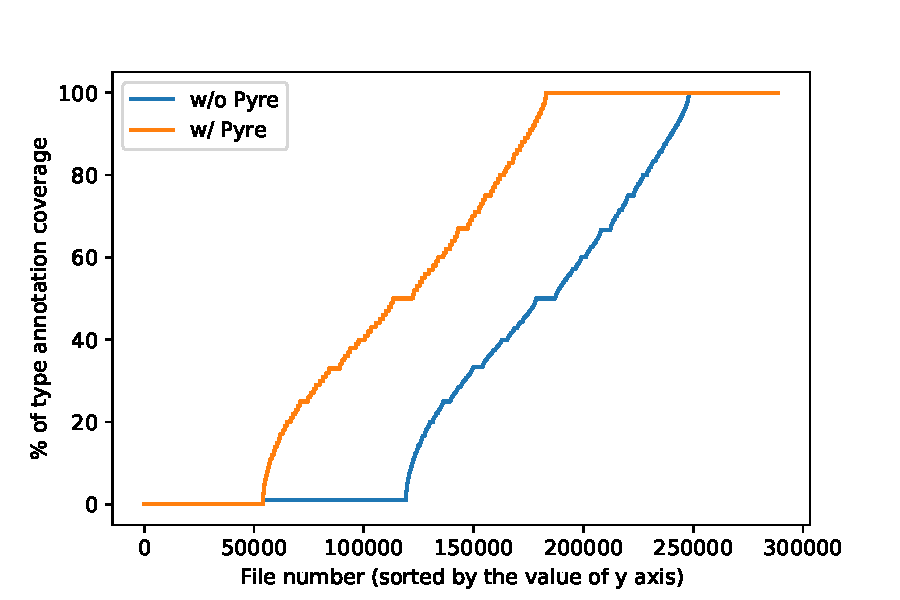
\includegraphics[width=\linewidth]{chapters/ch4/figs/type_cove_f_pyre.pdf}
	\caption{The effect of using Pyre on the type annotation coverage of source code files}
	\label{ch4:fig:dataset-type-annot-cove-pyre}
\end{figure}

\subsection{Type Checking}
Recent studies show that developer-provided types rarely type-check and Python projects may contain type-related defects~\cite{ore2018assessing, rak2020python, khan2021empirical}. Therefore, we believe that it is essential to type-check the dataset to eliminate noisy ground truth (i.e. incorrect type annotations). Not only noisy ground truth can be considered a threat to the validity of results but also it may make the discrimination of types in type clusters more difficult~\cite{garcia2015effect}. To clean the dataset from noisy ground truth, we perform basic analysis as follows:
\begin{itemize}
	\item First, we use mypy to type-check 288,760 source files in the dataset. Of which, 184,752 source files are successfully type-checked.
	\item Considering the remaining 104,008 source files, for further analysis, we ignore source files that cannot be type-checked further by mypy due to syntax error or other fatal exceptions. This amounts to 63,735 source files in the dataset.
	\item Given 40,273 source files with type errors, we remove one type annotation at a time from a file and run mypy. If it type-checks, we include the file. Otherwise, we continue this step up to 10 times. This basic analysis fixes 16,861 source files with type errors, i.e, 42\% of the given set of files.
\end{itemize}

\begin{table}[!t]
	\centering
	\caption{Characteristics of the dataset used for evaluation}
	\label{ch4:tab:dataset}
	\begin{threeparttable}
		\begin{tabular}{@{}ll@{}}
			\toprule
			Metrics\tnote{a,b} & Our dataset \\
			\midrule
			Repositories & 5,092 \\
			Files & 201,613 \\
			Lines of code\tnote{c} & 11.9M \\
			\midrule
			Functions & 882,657 \\
			...with return type annotations & 94,433 (10.7\%) \\
			\midrule
			Arguments & 1,558,566 \\
			...with type annotations & 128,363 (14.5\%) \\
			\midrule
			Variables & 2,135,361 \\
			...with type annotations & 1,023,328 (47.9\%) \\
			\midrule
			Types & 1,246,124 \\
			...unique & 60,333 \\
			\bottomrule
		\end{tabular}
		\begin{tablenotes}[flushleft]
			\item[a] {\footnotesize Metrics are counted after the ASTs extraction phase of our pipeline.}
			%\item[b] {\footnotesize Pyre's inferred types are considered in the metrics as well.}
			\item[c] {\footnotesize Comments and blank lines are ignored when counting lines of code.}
		\end{tablenotes}
	\end{threeparttable}
\end{table}

\begin{table}
	\centering
	\caption{Number of data points for train, validation and test sets}
	\label{ch4:tab:datapoints}
	\begin{tabular}{@{}l l l l@{}}
		\toprule
		%		& \multicolumn{3}{@{}c@{}}{Our dataset} \\
		%		\cmidrule{2-4}
		& Argument type & Return type & Variable type\\
		\midrule
		Training & 90,114  & 37,803 & 426,235 \\
		Validation & 9,387 & 3,932 & 48,518 \\
		Test & 24,121 & 10,444 & 118,319 \\
		\midrule
		Total &  108,888 (16.06\%) & 45,667 (6.74\%) & 523,271 (77.20\%) \\
		\bottomrule
		%		\vspace{6pt}\\
		%		\toprule
		%		& \multicolumn{2}{c}{Typilus' dataset \cite{allamanis2020typilus} } \\
		%		\cmidrule{2-3}
		%		& Argument type & Return type  \\
		%		\midrule
		%		Training & 60,574  & 23,227  \\
		%		Validation & 5,647  & 2,243 \\
		%		Test & 16,964 & 6,349 \\
		%		\midrule
		%		Total & 83,185 (72.3\%) & 31,819 (27.7\%) \\
		%		\bottomrule
	\end{tabular}
\end{table}

\subsection{Dataset Characteristics}
% Similar to \cite{allamanis2020typilus}, we used \texttt{PyType} to infer type annotations for the projects of the Typilus' dataset.
Table \ref{ch4:tab:dataset} shows the characteristics of our dataset after code de-duplication, augmentation, and type-checking. In total, there are more than 882K functions with around 1.5M arguments. Also, the dataset has more than 2.1M variable declarations. Of which, 48\% have type annotations.

Figure \ref{ch4:fig:top_10_types} shows the frequency of top 10 most frequent types in our dataset. It can be observed that types follow a long-tail distribution. Unsurprisingly, the top 10 most frequent types amount to 59\% of types in the dataset. Lastly, we randomly split the dataset by files into three sets: 70\% training data, 10\% validation data, and 20\% test data. Table \ref{ch4:tab:datapoints} shows the number of data points for each of the three sets.

\subsection{Pre-processing}
Similar to the previous work~\cite{pradel2019typewriter, allamanis2020typilus}, before training ML models, we have performed several pre-processing steps:

\begin{itemize}
	\item Trivial functions such as \code{\_\_str\_\_} and \code{\_\_len\_\_} are not included in the dataset. The return type of this kind of functions is straightforward to predict, i.e., \code{\_\_len\_\_} always returns \code{int}, and would blur the results.
	\item We excluded \code{Any} and \code{None} type annotations as it is not helpful to predict these types.
	\item We performed a simple type aliasing resolving to make type annotations of the same kind consistent. For instance, we map \code{[]} to \code{List}, \code{\{\}} to \code{Dict}, and \code{Text} to \code{str}.
	\item We resolved qualified names for type annotations. For example, \code{array} is resolved to \code{numpy.array}. This makes all the occurrences of a type annotation across the dataset consistent.
	\item Same as the work of Allamanis et al.~\cite{allamanis2020typilus}, we rewrote the components of a base type whose nested level is greater than 2 to \code{Any}. For instance, we rewrite \\ \code{List[List[Tuple[int]]]} to \code{List[List[Any]]]}. This removes very rare types or outliers.
\end{itemize}

\begin{figure}[!t]
	\centering
	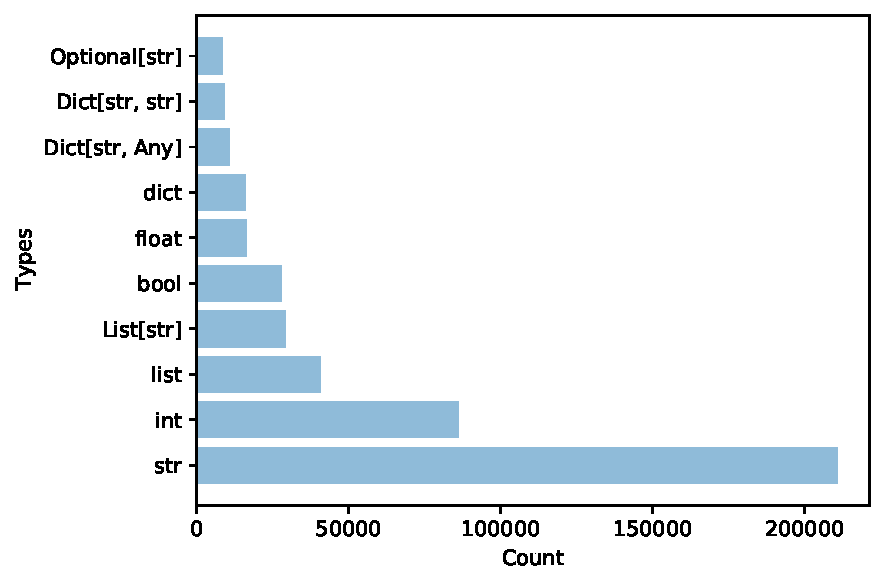
\includegraphics[width=\linewidth]{chapters/ch4/figs/top-10-most-frequent-types.pdf}
	\caption{Top 10 most frequent types (\texttt{Any} and \texttt{None} types are excluded)}
	\label{ch4:fig:top_10_types}
\end{figure}

\section{Evaluation Setup}\label{ch4:sec:es}
In this section, we describe the baseline models, the implementation details and the training of the neural models. Lastly, we explain evaluation metrics to quantitatively measure the performance of ML-based type inference approaches.

\subsection{Baselines}
We compare \name to Typilus~\cite{allamanis2020typilus} and TypeWriter~\cite{pradel2019typewriter}, which are recent state-of-the-art ML-based type inference approaches for Python. Considering Table \ref{tab:comp-learning-appr}, \name has an HNN-based neural model whereas Typilus's neural model is GNN-based. However, Typilus has the same prediction abilities as \name and has no limitation on the size of type vocabulary which makes it an obvious choice for comparison. Compared with \name, TypeWriter has two main differences. First, TypeWriter's type vocabulary is small and pre-defined (i.e. 1,000 types) at training time. Second, TypeWriter cannot predict the type of variables, unlike \name and Typilus.

\subsection{Implementation Details and Environment Setup}
\label{ch4:sub:implementation}
We implemented \name and TypeWriter in Python 3 and its ecosystem. We extract the discussed type hints from ASTs using LibSA4Py~\cite{libsa4py}. The data processing pipeline is parallelized by employing the \textit{joblib} package. We use NLTK \cite{loper2002nltk} for performing standard NLP tasks such as tokenization and stop work removal. To train the Word2Vec model, the \textit{gensim} package is used. For the neural model, we used bidirectional LSTMs \cite{schuster1997bidirectional} in the PyTorch framework \cite{paszke2019pytorch} to implement the two RNNs. Lastly, we used the Annoy\cite{annoy} package to perform a fast and approximate nearest neighbor search. For Typilus, we used its public implementation on GitHub \cite{typilus}.

We performed all the experiments on a Linux operating system (Ubuntu 18.04.5 LTS).
The computer had an AMD Ryzen Threadripper 1920X with 24 threads (@3.5GHz), 64 GB of RAM, and two NVIDIA GeForce RTX 2080 TIs.

\begin{table}[!t]
	\caption{Value of hyperparameters for neural models}
	\label{ch4:tab:hyperp}
	\begin{threeparttable}\begin{tabular}{@{}lrrr@{}}
				\toprule
				Hyperparameter &  \name & TypeWriter & Typilus \\
				\midrule
				Word embedding dimension (i.e. $d$) & 100 & 100 & N/A \\
				Size of visible type hints vocabulary (i.e. $T$) & 1024 & 1024 & N/A \\
				LSTM hidden nodes & 256 & 256 & N/A \\
				GNN hidden nodes & N/A & N/A & 64 \\
				Dimension of linear layer's output & 1536 & 1000 & N/A \\
				Number of LSTM's layers & 1 & 1 & N/A \\
				Learning rate & 0.002 & 0.002 & 0.00025 \\
				Dropout rate & 0.25 & 0.25 & 0.1 \\
				Number of epochs & 25 & 25 & 500\tnote{a} \\
				Batch size & 5864 & 4096 & N/A \\
				Value of $k$ for nearest neighbor search & 10 & N/A & 10 \\
				Tripet loss' margin value (i.e. $m$) & 2.0 & N/A & 2.0 \\
				\midrule
				Model's trainable parameters & 4.6M & 4.7M & 650K \\
				\bottomrule
			\end{tabular}
			\begin{tablenotes}
				\item[a] {\footnotesize The model stopped at epoch 38 due to the early stopping technique.}
			\end{tablenotes}
	\end{threeparttable}
\end{table}

\subsection{Training}
To avoid overfitting the train set, we applied the Dropout regularization \cite{srivastava2014dropout} to the input sequences except for the visible types. Also, we employed the Adam optimizer \cite{kingma2014adam} to minimize the value of the Triplet loss function. For both \name and TypeWriter, we employed the data parallelism feature of PyTorch to distribute training batches between the two GPUs with a total VRAM of 22 GB.  For the \name model, given 554K training samples, a single training epoch takes around 4 minutes. It takes 7 seconds for the TypeWriter model providing that its training set contains 127K training samples\footnote{Note that TypeWriter uses only argument and return samples as it lacks the variable prediction ability.}. Aside from the training sample size, \name is a DSL-based model and hence it has to predict the output of three data points for every single training batch (see Eq. \ref{eq:triplet}). Typilus completes a single training epoch in around 6 minutes\footnote{The public implementation of Typilus does not take advantage of our two GPUs.}. For all the neural models, the validation set is used to find the optimal number of epochs for training. The value of the neural models' hyperparameters is reported in Table \ref{ch4:tab:hyperp}.

\subsection{Evaluation Metrics}
We measure the type prediction performance of an approach by comparing the type prediction $t_{p}$ to the ground truth $t_{g}$ using two criteria originally proposed by Allamanis et al.~\cite{allamanis2020typilus}:

\begin{description}
	%
	\item[Exact Match:] $t_{p}$ and $t_{g}$ are exactly the same type.
	%
	\item[Base Type Match:] ignores all type parameters and only matches the base types.
	%That is, it matches the outermost of a parametric type.
	For example, \code{List[str]} and \code{List[int]} would be considered a match.
	%
\end{description}

In addition to these two criteria, as stated earlier, we opt for the MRR metric~\cite{manning2008introduction}, since the neural models predict a list of types for a given query. The MRR of multiple queries $Q$ is defined as follows:
\begin{equation}
MRR = \frac{1}{|Q|}\sum_{i=1}^{|Q|}{\frac{1}{r_{i}}}
\end{equation}
The MRR metric partially rewards the neural models by giving a score of $\frac{1}{r_{i}}$ to a prediction if the correct type annotation appears in rank $r$. Like Top-1 accuracy, a score of 1 is given to a prediction for which the Top-1 suggested type is correct. Hereafter, we refer to the MRR of the Top-$n$ predictions as MRR@$n$. We evaluate the neural models up to the Top-10 predictions as it is a quite common methodology in the evaluation of ML-based models for code~\cite{ he2021pyart, allamanis2020typilus, pradel2019typewriter}.

Similar to the evaluation methodology of Allamanis et al.~\cite{allamanis2020typilus}, we consider types that we have seen more than 100 times in the train set as \emph{common} or \emph{rare} otherwise. Additionally, we define the set of \emph{ubiquitous} types, i.e., $\{\texttt{str}, \texttt{int}, \texttt{list}, \texttt{bool}, \texttt{float}\}$. These types are among the top 10 frequent types in the dataset (see Fig.~\ref{ch4:fig:top_10_types}) and they are excluded from the set of common types. Furthermore, Unlike \name and Typilus, TypeWriter predicts \code{unknown} if the expected type is not present in its type vocabulary. Thus, to have a valid comparison with the other two approaches, we consider \code{other} predictions by TypeWriter in the calculation of evaluation metrics.

\newpage

\section{Evaluation}
\label{ch4:sec:eval}
% \NewDocumentCommand\RQ{m}{RQ$_{#1}$}

To evaluate and show the effectiveness of \name, we focus on the following research questions.

\begin{description}[noitemsep]
	\item[\RQ{1}] What is the general type prediction performance of \name? 
	%	\item[\RQ{2}] How does \name perform while considering different top-$n$ predictions?
	\item[\RQ{2}] How does \name perform while considering different predictions tasks?
	\item[\RQ{3}] How do each proposed type hint and the size of type vocabulary contribute to the performance of \name?
	%\item[\RQ{4}] How effective is \name in terms of training and inference speed?
	%\item[\RQ{5}] How does \name compare qualitatively to the other approaches?
\end{description}

\begin{table*}[!t]
	\centering
	\caption{Performance evaluation of the neural models considering different top-$n$ predictions}
	\label{ch4:tab:top-n}
	   \begin{threeparttable}
	\resizebox{\textwidth}{!}{\begin{tabular}{@{}l l c c c c c c c c c @{}}
		\toprule
		\multirow{2}{*}{Top-$n$ predictions} &  \multirow{2}{*}{Approach} & \multicolumn{4}{c}{\% Exact Match} & & \multicolumn{3}{c}{\% Base Type Match\tnote{a}} & \\
		\cmidrule{3-6} \cmidrule{8-10}
		& & All & Ubiquitous & Common & Rare & & All & Common & Rare & \\
		\midrule
		\multirow{3}{*}{Top-1}  & \name & \textbf{75.8} & \textbf{100.0} & \textbf{82.3} & 19.2 & & \textbf{80.6} & \textbf{85.2} & 36.0 &  \\
		& Typilus  & 66.1 & 92.5 & 73.4 & \textbf{21.6} & & 74.2 & 81.6 & \textbf{41.7} &  \\
		& TypeWriter & 56.1 & 93.5 & 60.9 & 16.2 & & 58.3 & 64.4 & 19.9 & \\
		& & & & & & & & & & \\
		\multirow{3}{*}{Top-3}  & \name & \textbf{78.1} & \textbf{100.0} & \textbf{87.3} & 23.4 & & \textbf{83.8} & \textbf{90.6} & 43.2 &  \\
		& Typilus & 71.6 & 96.2 & 83.0 & \textbf{26.8} & & 79.8 & 88.7 & \textbf{49.2} &  \\
		& TypeWriter  & 63.7 & 98.8 & 79.2 & 20.8 & & 67.3 & 83.5 & 27.9 & \\
		& & & & & & & & & & \\
		\multirow{2}{*}{Top-5}  & \name & \textbf{78.7} & \textbf{100.0} & \textbf{88.6} & 24.5 & & \textbf{84.7} & \textbf{92.1} & 45.5 & \\
		& Typilus & 72.7 & 96.7 & 85.1 & \textbf{28.2} & & 80.9 & 90.1 & \textbf{51.0} & \\
		& TypeWriter & 65.9 & 99.6 & 84.9 & 23.0 & & 70.4  & 89.1 & 32.1 &  \\
		& & & & & & & & & &  \\
		\multirow{2}{*}{Top-10}  &\name & \textbf{79.2} & \textbf{100.0} & 89.7 & 25.2 & & \textbf{85.4} & \textbf{93.3} & 46.9 &   \\
		& Typilus  & 73.3 & 97.04 & 86.4 & \textbf{28.9} & & 81.5 & 90.9 & \textbf{51.9} &  \\
		& TypeWriter & 68.2 & 99.9 & \textbf{90.8} & 25.5 & & 73.2 & 93.8 & 36.5 &  \\
		\midrule
		\multirow{3}{*}{MRR@10} & \name & \textbf{77.1} & \textbf{100.0} & \textbf{85.1} & 21.4 & & \textbf{74.1} & \textbf{79.9} & 29.4 &  \\
		& Typilus  & 69.0 & 94.4 & 78.5 & \textbf{24.4} & & 67.4 & 75.8 & \textbf{32.8} & \\
		& TypeWriter & 60.4 & 96.1 & 71.3 & 19.1 & & 56.5 & 68.0 & 19.7 & \\
		\bottomrule
	\end{tabular}}
	\begin{tablenotes}
		\item[a] {\footnotesize Ubiquitous types are not a base type match. However, they are considered in the All column.}
	\end{tablenotes}
\end{threeparttable}
\end{table*}

\subsection{Type Prediction Performance (\textbf{RQ}$_{1}$)}
\label{ch4:sub:quanti-eval}
In this subsection, we compare our proposed approach, \name, with the selected baseline models in terms of overall type prediction performance.

\paragraph{Method}
The models get trained on the training set and the test set is used to measure the type prediction performance.
We evaluate the neural models by considering different top-$n$ predictions, i.e., $n=\{1,3,5,10\}$.
Also, for this RQ, we consider all the supported inference tasks by the models, i.e., arguments, return types, and variables.

\paragraph{Results}
Table \ref{ch4:tab:top-n} shows the overall performance of the neural models while considering different top-$n$ predictions. Given the Top-10 prediction, \name outperforms both Typilus and TypeWriter based on both the exact and base type match criteria (all). Specifically, considering the exact match criteria (all types), \name performs better than Typilus and TypeWriter at the Top-10 prediction by a margin of 5.9\% and 11\%, respectively. Moreover, it can be seen that the \name's performance drop is less significant compared to the other two models when decreasing the value of $n$ from Top-10 to Top-1. For instance, by considering Top-1 rather than Top-10 and the exact match criteria (all), the performance of \name, Typilus, and TypeWriter drop by 3.4\%, 7.2\%, 12.1\%, respectively. Concerning the prediction of rare types, Typilus slightly performs better than \name, which can be attributed to the use of an enhanced triplet loss function. It is also worth mentioning that \name achieves a 100\% exact match for the ubiquitous types at Top-1, which is remarkable.

\begin{figure}[!t]
	\centering
	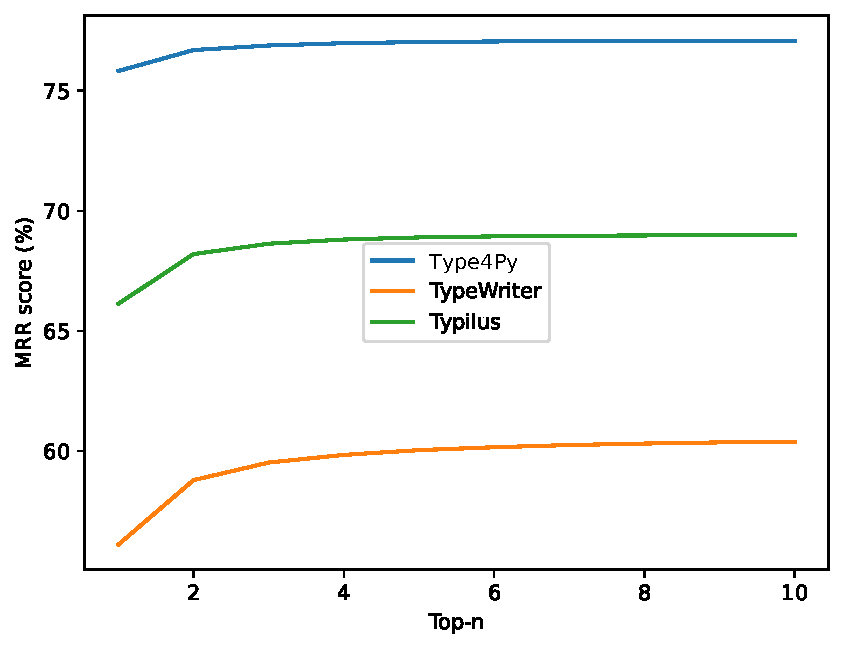
\includegraphics[width=0.75\linewidth]{chapters/ch4/figs/top-n-MRR.pdf}
	\caption{The MRR score of the models considering different top-$n$ predictions}
	\label{ch4:fig:top-n-MRR}
\end{figure}

As stated earlier, developers are more likely to use the first suggestion by a tool~\cite{parnin2011automated}. Therefore, we evaluated the neural models by the MRR@10 metric at the bottom of Table \ref{ch4:tab:top-n}. Ideally, the difference between the MRR@10 metric and the Top-1 prediction should be zero. However, this is very challenging as the neural models are not 100\% confident in their first suggestion for all test samples. Given the results of MRR@10, we observe that \name outperforms both Typilus and TypeWriter by a margin of 8.1\% and 16.7\%, respectively. In addition, we investigated the MRR score of the neural models while considering different values of Top-$n$, which is shown in Figure \ref{ch4:fig:top-n-MRR}. As can be seen, \name has a substantially higher score than the other models across all values of $n$. Moreover, the MRR score of all the three neural models almost converges to a fixed value after MRR@3. Given the findings of the RQ1, we use MRR@10 and the Top-1 prediction for the rest of the evaluation as we believe this better shows the practicality of the neural models for assisting developers.

\begin{table*}[!t]
	\centering
	\caption{Performance evaluation of the neural models considering different tasks}
	\label{ch4:tab:different-tasks}
	\begin{threeparttable}
		\resizebox{\textwidth}{!}{\begin{tabular}{@{}l l l c c c c c c c c c @{}}
			\toprule
			\multirow{2}{*}{Metric} & \multirow{2}{*}{Task} &  \multirow{2}{*}{Approach} & \multicolumn{4}{c}{\% Exact Match} & & \multicolumn{3}{c}{\% Base Type Match}& \\
			\cmidrule{4-7} \cmidrule{9-11}
			& & & All & Ubiquitous & Common & Rare & & All & Common & Rare & \\
			\midrule
			\multirow{10}{*}{Top-1 prediction} & \multirow{3}{*}{Argument} & \name & \textbf{61.9} & \textbf{100.0} & \textbf{64.5} & 17.4 & & \textbf{63.9} & \textbf{69.3} & 20.1 & \\
			& & Typilus  & 53.8 & 83.3 & 46.6 & \textbf{23.7} & & 57.0 & 52.5 & \textbf{29.6} & \\
			& & TypeWriter & 58.4 & 93.6 & 61.3 & 19.6 & & 60.1 & 64.4 & 22.1 & \\
			& & & & & & & & & & & \\
			& \multirow{3}{*}{Return}  & \name & \textbf{56.4} & \textbf{100.0} & 59.3 & \textbf{14.4} & & \textbf{60.3} & \textbf{65.4} & 20.9 & \\
			& & Typilus  & 42.5 & 84.0 & 41.6 & 12.3 & & 49.9 & 49.5 & \textbf{24.8} & \\
			& & TypeWriter  & 50.7 & 93.3 & \textbf{59.9} & 9.2 & & 54.1 & 64.4 & 15.0 & \\
			& & & & & & & & & & & \\
			& \multirow{2}{*}{Variable\tnote{a}}  & \name & \textbf{80.4} & \textbf{100.0} & \textbf{86.8} & 20.7 & & \textbf{85.9} & \textbf{89.1} & 44.6 & \\
			& & Typilus & 71.4 & 95.1 & 80.5 & \textbf{22.5} & & 80.7 & \textbf{89.1} & \textbf{48.6} & \\
			& & & & & & & & & & & \\
			\multirow{10}{*}{MRR@10} & \multirow{3}{*}{Argument} & \name & \textbf{64.2} & \textbf{100.0} & 69.5 & 20.7 & & \textbf{59.9} & 62.2 & 20.6 &  \\
			& & Typilus  & 58.7 & 87.9 & 55.4 & \textbf{27.5} & & 56.0 & 52.2 & \textbf{28.1} & \\
			& & TypeWriter & 63.3 & 96.2 & \textbf{72.4} & 23.0 & & 59.6 & \textbf{69.3} & 22.7 & \\
			& & & & & & & & & & &  \\
			& \multirow{3}{*}{Return}  & \name & \textbf{57.9} & \textbf{100.0} & 63.3 & \textbf{16.1} & & \textbf{52.9} & 55.8 & 18.5 & \\
			& & Typilus  & 46.0 & 86.9 & 49.8 & 14.3 & & 44.9 & 46.6 & \textbf{21.4} & \\
			& & TypeWriter  & 54.2 & 95.9 & \textbf{68.9} & 10.9 & & 49.9 & \textbf{65.1} & 14.2 & \\
			& & & & & & & & & & & \\
			& \multirow{2}{*}{Variable\tnote{a}}  & \name & \textbf{81.4} & \textbf{100.0} & \textbf{89.1} & 22.7 & & \textbf{79.1} & \textbf{85.0} & 34.1 & \\
			& & Typilus & 73.7 & 96.3 & 84.7 & \textbf{25.1} & & 72.4 & 82.7 & \textbf{36.1} & \\
			\bottomrule
		\end{tabular}}
		\begin{tablenotes}
			\item[a] {\footnotesize Note that TypeWriter cannot predict the type of variables.}
		\end{tablenotes}
	\end{threeparttable}
\end{table*}

\subsection{Different Prediction Tasks (\textbf{RQ}$_{2}$)}
Here, we compare \name with other baselines while considering different prediction tasks, i.e., arguments, return types, and variables.

\paragraph{Method}
Similar to the \RQ{1}, the models are trained and tested on the entire training and test sets, respectively.
However, we consider each prediction task separately while evaluating the models at Top-1 and MRR@10.

\paragraph{Results}
Table \ref{ch4:tab:different-tasks} shows the type prediction performance of the approaches for the three considered prediction tasks. In general, considering the exact match criteria (all), \name outperforms both Typilus and TypeWriter in all prediction tasks at both Top-1 and MRR@10. For instance, considering the return task and Top-1, \name obtains 56.4\% exact matches (all), which is 13.9\% and 5.7\% higher than that of Typilus and TypeWriter, respectively. Also, for the same task, the \name's MRR@10 is 11.9\% and 3.7\% higher compared to Typilus and TypeWriter, respectively. However, concerning the prediction of common types and MRR@10, TypeWriter performs better than both \name and Typilus at the argument and return tasks. This might be due to the fact that TypeWriter predicts from the set of 1,000 types, which apparently makes it better at the prediction of common types. Moreover, both \name and Typilus have a much larger type vocabulary and hence they need more training samples to generalize better providing that both argument and return types together amount to 22.8\% of all the data points in the dataset (see Table~\ref{ch4:tab:datapoints}). Lastly, in comparison with Typilus, \name obtains 7.7\% and 6.7\% higher MRR@10 score for the exact and base type match criteria (all), respectively.

\begin{table*}[!t]
	\centering
	\caption{Performance evaluation of \name with different configurations}
	\label{ch4:tab:models-different-configs}
	\resizebox{\textwidth}{!}{\begin{tabular}{@{}l l c c c c c c c c c @{}}
		\toprule
		\multirow{2}{*}{Metric} & \multirow{2}{*}{Approach} & \multicolumn{4}{c}{\% Exact Match} & & \multicolumn{3}{c}{\% Base Type Match\tnote{a}} & \\
		\cmidrule{3-6} \cmidrule{8-10}
		& & All & Ubiquitous & Common & Rare & & All & Common & Rare & \\
		\midrule
		\multirow{5}{*}{Top-1 prediction} & \name & \textbf{75.8} & \textbf{100.0} & 82.3 & \textbf{19.2} & & \textbf{80.6} & 85.2 & \textbf{36.0} & \\		
		& \name (w/o identifiers) & 72.7 & \textbf{100.0} & 71.8 & 17.4 & & 76.5 & 73.9 & 30.9 & \\
		& \name (w/o code context) & 67.9 & \textbf{100.0} & 59.2  & 11.4 & & 70.6 & 63.3 & 17.9 & \\
		& \name (w/o visible type hints)  & 65.4  & 86.2  & 71.9 & 15.8 & & 70.0 & 74.9 & 31.5 & \\
		& \name (w/ top 1,000 types)  & 74.5  & \textbf{100.0}  & \textbf{83.3} & 12.9 & & 79.1 & \textbf{86.3} & 28.5 & \\
		& & & & & & & & & & \\
		\multirow{5}{*}{MRR@10} & \name & \textbf{77.1} & \textbf{100.0} & 85.1  & \textbf{21.4} & & \textbf{74.1} & 79.9 & \textbf{29.4} & \\		
		& \name (w/o identifiers) & 73.8 & \textbf{100.0} & 74.6 & 19.2 & & 69.3 & 66.6 & 25.1 & \\
		& \name (w/o code context) & 69.7 & \textbf{100.0} & 63.9  & 13.6 & & 63.8 & 55.4 & 17.7 & \\
		& \name (w/o visible type hints) & 68.6  & 89.3 & 76.2 & 18.2 & & 65.8 & 70.1 & 26.2 & \\
		& \name (w/ top 1,000 types)  & 75.6  & \textbf{100.0}  & \textbf{86.2} & 14.2 & & 72.4 & \textbf{81.7} & 22.8 & \\
		\bottomrule
	\end{tabular}}
\end{table*}

\subsection{Ablation Analysis (\textbf{RQ}$_{3}$)}
\label{subsec:abalation}
Here, we investigate how each proposed type hint and the size of type vocabulary contribute to the overall performance of \name.

\paragraph{Method}
For ablation analysis, we trained and evaluated \name with 5 different configurations, i.e., (1) complete model (2) w/o identifiers (3) w/o code context (4) w/o visible type hints (5) w/ a vocabulary of top 1,000 types. Similar to the previous RQs, we measure the performance of \name with the described configurations at Top-1 and MRR@10.

\paragraph{Results}
Table \ref{ch4:tab:models-different-configs} presents the performance of \name with the five described configurations. It can be observed that all three type hints contribute significantly to the performance of \name. Code context has the most impact on the model's performance compared to the other two type hints. For instance, when ignoring code context, the model's exact match score for common types drops significantly by 23.1\%. After code context, visible type hints have a large impact on the performance of the model. By ignoring VTH, the model's exact match for ubiquitous types reduces from 100\% to 86.2\%. Although the Identifiers type hint contributes substantially to the prediction of common types, it has a less significant impact on the overall performance of \name compared to code context and VTH. In summary, we conclude that code context and VTH are the strongest type hints for our type prediction model.

By limiting the type vocabulary of \name to the top 1,000 types, similar to TypeWriter, we observe that the model's performance for common types is slightly improved while its performance for rare types is reduced significantly, i.e., 7.2\% considering MRR@10. This is expected as the model's type vocabulary is much smaller compared to the complete model's.

\begin{figure*}[!t]
	\centering
	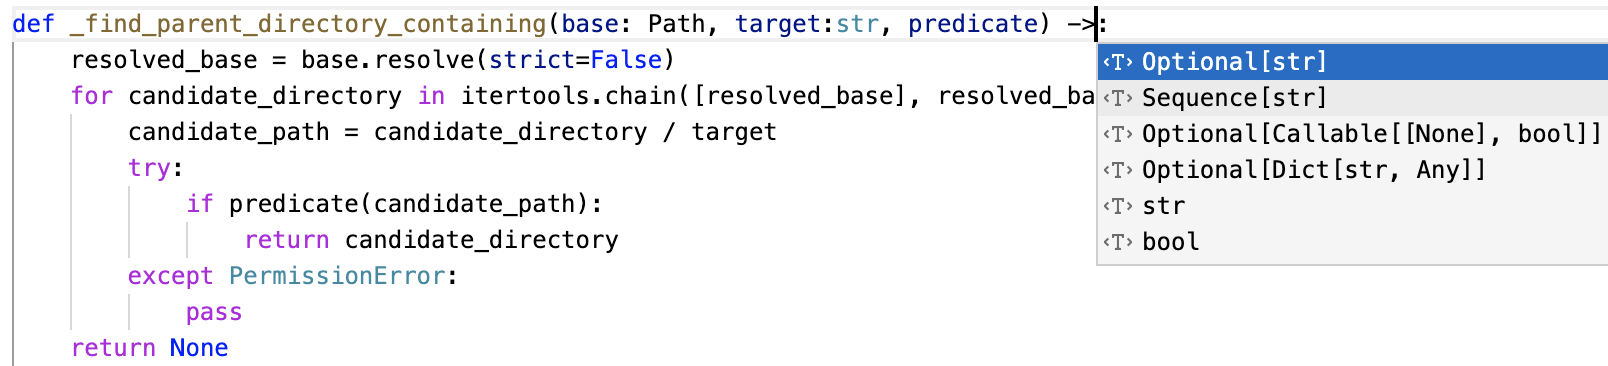
\includegraphics[width=\textwidth]{chapters/ch4/figs/VSC-IDE-pred.png}
	\caption{A type auto-completion example from VSC. The code has not been seen during training. The expected return type is \code{Optional[str]}.}
	\label{ch4:fig:VSC-IDE}
\end{figure*}

\section{Type4Py in Practice}\label{ch4:sec:prac}
To make the \name model practical, we developed an end-to-end solution including a web server and a Visual Studio Code (VSC) extension. We deployed this as an openly accessible web service that serves requests from the VSC extension. In this section, we describe the deployment components of \name.

\subsection{Deployment}
To deploy the pre-trained \name model for production, we convert the \name's PyTorch model to an ONNX model \cite{onnxruntime} which enables querying the model on both GPUs and CPUs with faster inference speed. Thanks to Annoy \cite{annoy}, a fast and memory-efficient KNN search is performed to suggest type annotations from type clusters.

\subsection{Web Server}
We have implemented a small Flask application to handle concurrent type prediction requests from users with Nginx as a proxy. This enables us to have quite a number of asynchronous workers that have an instance of \name’s ONNX model plus Type Clusters each. Specifically, the web application receives a Python source file via a POST request, queries an instance of the model, and finally it gives the file's predicted type annotations as a JSON response.

% TODO: Update No. of installation for the extension
\subsection{Visual Studio Code Extension}
As stated earlier, retrofitting type annotations is a daunting task for developers. To assist developers with this task, we have released a Visual Studio Code extension for \name~\cite{vscodet4py}, which uses the web server's API to provide ML-based type auto-completion for Python code. Figure \ref{ch4:fig:VSC-IDE} shows an example of a type recommendation from the VSC IDE. As of this writing, the extension has 909 installs on the Visual Studio Marketplace. Based on the user's consent, the VSC extension gathers telemetry data for research purposes. Specifically, accepted types, their rank in the list of suggestions, type slot kind, identifiers' name, and identifiers' line number are captured from the VSC environment and sent to our web server. In addition, rejected type predictions are captured when a type auto-completion window is closed without accepting a type.

By analyzing the gathered telemetry data from Jul. '21 to Aug. '21 and excluding the author(s), of 26 type auto-completion queries, 19 type annotations were accepted by the extension's users. Moreover, the average of accepted type annotations per developer is 69.6\%. Given that the gathered telemetry data is pretty small, we cannot draw a conclusion regarding the performance of \name in practice. However, our telemetry infrastructure and concerted efforts to broaden the user base will enable us to improve \name in the future.

\section{Discussion and Future Work}\label{ch4:sec:discuss}
Based on the formulated RQs and their evaluation in Section \ref{ch4:sec:eval}, we provide the following remarks:
\begin{itemize}
	%\setlength\itemsep{-0.2em}
	\item We used Pyre~\cite{pyre}, a static type inference tool, to augment our dataset with more type annotations. However, this can be considered as a \emph{weakly} supervision learning problem~\cite{zhou2018brief}, meaning that inferred types by the static tool might be noisy or imprecise despite the pre-processing steps. To eliminate this threat, we employed a static type checker, mypy, to remove source files with type errors from our dataset. Future work can devise a guided-search analysis to fix type errors in source files, which may improve the fix rate.
	
	\item It would be ideal for ML-based models to give a correct prediction in their first few suggestions, preferably Top-1, as developers tend to use the first suggestion by a tool~\cite{parnin2011automated}. Therefore, different from previous work on ML-based type prediction~\cite{pradel2019typewriter, allamanis2020typilus}, we use the MRR metric in our evaluation. We believe that the MRR metric better demonstrates the potential and usefulness of ML models to be used by developers in practice. Overall, considering the MRR metric, \name significantly outperforms the state-the-art ML-based type prediction models, namely, Typilus and TypeWriter.
	
	\item Considering the overall type prediction performance (\RQ{1}), both \name and Typilus generally perform better than TypeWriter. 
	This could be attributed to the fact that the two models map types into a
	high-dimensional space (i.e. type clusters). Hence this not only enables a much
	larger type vocabulary but also significantly improves their overall performance, especially the prediction
	of rare types.
	
	\item Given the results of \RQ{1} and \RQ{2}, our HNN-based neural model, \name, has empirically shown to be more effective than the GNN-based model of Typilus. We attribute this to the inherent bottleneck of GNNs which is over-squashing information into a fixed-size vector \cite{alon2020bottleneck} and thus they fail to capture long-range interaction. However, our HNN-based model concatenates learned features into a high-dimensional vector and hence it preserves information and its long-range dependencies.
	
	\item According to the results of ablation analysis (\RQ{3}), the three
	proposed type hints, i.e., identifiers, code context, and VTHs are
	all effective and positively contribute to the performance of \name. This result does not come
	at the expense of generalizability; our visible type analysis is not more
	sophisticated than what an IDE like PyCharm or VSCode do to determine
	available types for, e.g., auto-completion purposes.
	
	%	\item As indicated in the qualitative evaluation (\RQ{5}), the HNN-based model
	%    of \name has a better discriminative ability than the GNN-based model of Typilus, which results in a substantially higher type prediction performance. We attribute this to the inherent bottleneck of GNNs which is over-squashing information into a fixed-size vector \cite{alon2020bottleneck} and thus they fail to capture long-range interaction. However, our HNN-based model concatenates learned features into a high-dimensional vector and hence it preserves information and its long-range dependencies.
	
	\item Both \name and Typilus cannot make a correct prediction for types beyond their
	pre-defined (albeit very large) type clusters. For example, they currently cannot
	synthesize types, meaning that they will never suggest a type such as
	\texttt{Optional[Dict[str, int]]} if it does not exist in their type clusters.
	To address this, future research can explore pointer networks~\cite{vinyals2015pointer} or a GNN model that captures type system rules.
	
	\item We believe that \name's VSC extension is one step forward towards improving developers' productivity by using machine-aided code tools. 
	In this case, the VSC extension aids Python developers to retrofit types for their existing codebases. After gathering sufficiently large telemetry data from the usage of \name, we will study how to improve \name's ranking and quality of predictions for, ultimately, a better user experience.
\end{itemize}

\section{Summary}\label{ch4:sec:sum}
In this chapter, we present \name, a DSL-based hierarchical neural network type inference model for Python. It considers identifiers, code context, and visible type hints as features for learning to predict types. Specifically, the neural model learns to efficiently map types of the same kind into their own clusters in a high-dimensional space, and given type clusters, the $k$-nearest neighbor search is performed to infer the type of arguments, variables, and functions' return types. We used a type-checked dataset with sound type annotations to train and evaluate the ML-based type inference models. Overall, the results of our quantitative evaluation show that the \name model outperforms other state-of-the-art approaches. Most notably, considering the MRR@10 score, our proposed approach achieves a significantly higher score than that of Typilus and TypeWriter's by a margin of 8.1\% and 16.7\%, respectively. This indicates that our approach gives a more relevant prediction in its first suggestion, i.e., Top-1. Finally, we have deployed \name in an end-to-end fashion to provide ML-based type auto-completion in the VSC IDE and aid developers in retrofitting type annotations for their existing codebases.